%%%%%%%%%%%%%%%%%%%%%%%%%%%%%%%%%%%%%%%%%
% Beamer Presentation
% LaTeX Template
% Version 1.0 (10/11/12)
%
% This template has been downloaded from:
% http://www.LaTeXTemplates.com
%
% License:
% CC BY-NC-SA 3.0 (http://creativecommons.org/licenses/by-nc-sa/3.0/)
%
%%%%%%%%%%%%%%%%%%%%%%%%%%%%%%%%%%%%%%%%%

%----------------------------------------------------------------------------------------
%	PACKAGES AND THEMES
%----------------------------------------------------------------------------------------

\documentclass[11pt]{beamer}

\usepackage[IL2]{fontenc}
\usepackage[utf8]{inputenc}

\usepackage[english]{babel}

%\mode<presentation> {

% The Beamer class comes with a number of default slide themes
% which change the colors and layouts of slides. Below this is a list
% of all the themes, uncomment each in turn to see what they look like.

%\usetheme{default}
%\usetheme{AnnArbor}
%\usetheme{Antibes}
%\usetheme{Bergen}
%\usetheme{Berkeley}
%\usetheme{Berlin}
%\usetheme{Boadilla}
%\usetheme{CambridgeUS}
%\usetheme{Copenhagen}
%\usetheme{Darmstadt}
%\usetheme{Dresden}
%\usetheme{Frankfurt}
%\usetheme{Goettingen}
%\usetheme{Hannover}
%\usetheme{Ilmenau}
%\usetheme{JuanLesPins}
%\usetheme{Luebeck}
%\usetheme{Madrid}
%\usetheme{Malmoe}
%\usetheme{Marburg}
%\usetheme{Montpellier}
\usetheme[progressbar = frametitle]{metropolis}

\makeatletter
\setlength{\metropolis@titleseparator@linewidth}{1.0pt}
\setlength{\metropolis@progressonsectionpage@linewidth}{1.0pt}
\setlength{\metropolis@progressinheadfoot@linewidth}{1.0pt}
\makeatother

%\usetheme{PaloAlto}
%\usetheme{Pittsburgh}
%\usetheme{Rochester}
%\usetheme{Singapore}
%\usetheme{Szeged}
%\usetheme{Warsaw}

% As well as themes, the Beamer class has a number of color themes
% for any slide theme. Uncomment each of these in turn to see how it
% changes the colors of your current slide theme.

%\usecolortheme{albatross}
%\usecolortheme{beaver}
%\usecolortheme{beetle}
%\usecolortheme{crane}
%\usecolortheme{dolphin}
%\usecolortheme{dove}
%\usecolortheme{fly}
%\usecolortheme{lily}
%\usecolortheme{orchid}
%\usecolortheme{rose}
%\usecolortheme{seagull}
%\usecolortheme{seahorse}
%\usecolortheme{whale}
%\usecolortheme{wolverine}

%\setbeamertemplate{footline} % To remove the footer line in all slides uncomment this line
%\setbeamertemplate{footline}[page number] % To replace the footer line in all slides with a simple slide count uncomment this line

%\setbeamertemplate{navigation symbols}{} % To remove the navigation symbols from the bottom of all slides uncomment this line
%}

\usepackage{lmodern}
\usepackage{mathpazo}

\usepackage{graphicx} % Allows including images
%\usepackage[czech]{babel}
%\usepackage[T1]{fontenc}
%\usepackage{amsmath}
%\usepackage{amsfonts}
%\usepackage{amssymb}
%\usepackage{amsthm}
\usepackage{array}
\usepackage{mathrsfs}


\usepackage{tikz}

\usetikzlibrary{arrows,calc,patterns}
\usetikzlibrary{decorations.pathreplacing,decorations.markings}
\usepackage{pgfplots}

\usepackage{animate}
%\usepackage{movie15}
\usepackage{appendixnumberbeamer}

\usepackage{bibentry}  

\nobibliography*


\newcommand{\Cbb}{\mathbb{C}}
\newcommand{\Rbb}{\mathbb{R}}
\newcommand{\Zbb}{\mathbb{Z}}
\newcommand{\Nbb}{\mathbb{N}}
%\setlength\parindent{0pt}

\newcommand{\D}[1]{\ensuremath{\operatorname{d}\!{#1}}}
\newcommand{\dif}[3][]{\frac{\D{{}^{#1}#2}}{\D{#3}^{#1}}}
\newcommand{\pardif}[3][]{\frac{\partial^{#1}{#2}}{\partial{#3}^{#1}}}
\newcommand{\pardift}[3]{\left(\pardif{#1}{#2}\right)_{#3}}
\newcommand{\difs}[3][]{\partial_{#3}^{#1}{#2}}
\newcommand{\op}[1]{\ensuremath{\hat{\mathbf{#1}}}}
\newcommand{\mat}[1]{\ensuremath{\ifnum\pdfstrcmp{#1}{1}=0 \mathbb{1}\else \mathbf{#1}\fi}}
\newcommand{\bra}[1]{\langle #1 \vert}
\newcommand{\ket}[1]{\vert #1 \rangle}
\newcommand{\bralr}[1]{\langle #1 \vert}
\newcommand{\ketlr}[1]{\vert #1 \rangle}
\newcommand{\braketlr}[2]{\left\langle\left. #1\right\vert #2\right\rangle}
\newcommand{\braket}[2]{\langle #1\vert #2\rangle}
\DeclareMathOperator{\tr}{\operatorname{tr}}
\newcommand{\abs}[1]{{\left\vert #1\right\vert}}
\newcommand{\mean}[1]{{\left\langle #1\right\rangle}}
\newcommand{\un}[1]{\,\mathrm{#1}}
\newcommand{\me}{\mathrm{e}}
\newcommand{\mi}{\mathrm{i}}
\newcommand{\lp}{\left(}
\newcommand{\rp}{\right)}
\newcommand{\at}[2]{\left. #1 \right\vert_{#2}}

\newcommand{\hatx}{\hat{X}}
\newcommand{\prim}[1]{{#1}^{\prime}}



\setbeamerfont{title}{size=\LARGE,%
	series=\bfseries}
\setbeamerfont{author}{size=\normalsize}
\setbeamerfont{date}{size=\normalsize}

\setbeamerfont{institute}{size=\footnotesize}





%----------------------------------------------------------------------------------------
%	TITLE PAGE
%----------------------------------------------------------------------------------------

\title[Classical string motion]{Classical string motion} % The short title appears at the bottom of every slide, the full title is only on the title page

\author{Vojtěch Liška} % Your name
\institute[PřF MUNI] % Your institution as it will appear on the bottom of every slide, may be shorthand to save space
{
Masaryk University, Faculty of Science \\ % Your institution for the title page
\medskip
\scriptsize{Supervisor: prof. Rikard von Unge}
%\textit{john@smith.com} % Your email address
}

\date{June 11, 2019}

\titlegraphic{\vspace{5.0cm}\flushright\includegraphics[height=2.0cm]{sci_lg_eng_cmyk.pdf}}

\begin{document}


\begin{frame}[plain]
	\titlepage % Print the title page as the first slide
\end{frame}

%\begin{frame}
%	\frametitle{Přehled} % Table of contents slide, comment this block out to remove it
%	\tableofcontents % Throughout your presentation, if you choose to use \section{} and \subsection{} commands, these will automatically be printed on this slide as an overview of your presentation
%\end{frame}

%----------------------------------------------------------------------------------------
%	PRESENTATION SLIDES
%----------------------------------------------------------------------------------------

%------------------------------------------------
%\section{Multimode optical fibre} % Sections can be created in order to organize your presentation into discrete blocks, all sections and subsections are automatically printed in the table of contents as an overview of the talk
%------------------------------------------------

%\subsection{Subsection Example} % A subsection can be created just before a set of slides with a common theme to further break down your presentation into chunks
%\section{Introduction to propagation in optical fibres}

\begin{frame}
	\frametitle{Objectives}
		Find explicit solutions of classical relativistic strings on various backgrounds, specifically:
		\begin{itemize}
			\item constantly expanding universe -- de Sitter spacetime
			\item gravitational wave background
			\item interaction with gravitational wave pulse
		\end{itemize}
\end{frame}



\begin{frame}
	\frametitle{Strings vs. particles}
	\begin{tikzpicture}
	\begin{axis}[
	hide axis,
	view = {20}{20},
	xscale = 0.5,
	yscale = 1.0
	]
	\addplot3[variable=t,
	mesh,
	colormap/greenyellow,
	samples = 50,
	ultra thick,
	domain=0:1] ({exp(t)*cos(70*t)}, {exp(t)*sin(70*t)}, t);
	\end{axis}
	\end{tikzpicture} \hspace{1.8cm}
	\begin{tikzpicture}
	\begin{axis}[
	hide axis,
	view = {20}{20},
	xscale = 0.6,
	yscale = 1.1
	]
	\addplot3 [
	surf,
	colormap/greenyellow, 
	%shader     = flat,
	point meta = z,
	samples    = 30,
	samples y  = 15,
	z buffer   = sort,
	domain     = 0:360,
	y domain   =-4:4
	] (
	{cosh(y/4)*cos(x)},
	{cosh(y/4)*sin(x)},
	{y}
	);
	\end{axis}
	\end{tikzpicture} \hspace{1.8cm}
	\begin{tikzpicture}
	\begin{axis}[
	hide axis,
	view = {20}{20},
	xscale = 0.5,
	yscale = 1.2
	]
	\addplot3 [
	surf,
	colormap/greenyellow,
	%shader     = faceted interp,
	point meta = z,
	samples    = 15,
	samples y  = 15,
	z buffer   = sort,
	domain     = 0:2,
	y domain   =-1:1
	] (
	{-x},
	{-(x^2-y^2)/2},
	{y}
	);
	\end{axis}
	\end{tikzpicture}
	
\end{frame}



\begin{frame}
	\frametitle{Nambu-Goto action for strings}
	\begin{itemize}
		\item Action in terms of induced metric on string worldsheet:
		$$		
			S = -T \int\limits_{0}^{\sigma_1} \int\limits_{\tau_i}^{\tau_f} \D \sigma \D \tau \sqrt{-\det \gamma}
		$$
		where $\tau$ and $\sigma$ are parametric coordinates on the worldsheet.
		\item $\gamma$ in spacetime coordinates $X$:
		$$
			\gamma_{\alpha \beta} = g_{M N}~ \difs[]{X^M}{\alpha}  ~ \difs[]{X^N}{\beta} 
		$$
		\item Good choice of parameterization can greatly simplify the~equations of motion.
		\end{itemize}
\end{frame}

\section{Flat spacetime}


\begin{frame}
	\frametitle{Flat spacetime}
	\begin{itemize}
		\item Minkowski spacetime -- with the right choice of parameterization
		$$
		\gamma_{\tau \tau} + \gamma_{\sigma \sigma} = 0, \qquad \gamma_{\tau \sigma} = \gamma_{\sigma \tau} = 0,
		$$
		the equations of motion become the wave equation:
		$$
		\difs[2] {X^M} {\tau} - \difs[2] {X^N} {\sigma} = 0
		$$
		\pause
		\item Closed strings have to be $\sigma_1$ periodic in $\sigma$ -- solutions can be expressed as a superposition of modes (eigenstates):
		$$
		X^{M}(\tau, \sigma) = \sum\limits_{k \in \Zbb} X_k^M(\tau) \me^{2 \pi \mi k \sigma / \sigma_1 },
		$$
		where the evolution in $\tau$ of each mode is just 
		$$
		X_k^M(\tau) = A^M \me^{2 \pi \mi k \tau / \sigma_1 } + B^M \me^{-2 \pi \mi k \tau / \sigma_1 }
		$$
	\end{itemize}
\end{frame}


\begin{frame}
	\frametitle{Flat spacetime}
	\begin{center}
	\animategraphics[autoplay,loop,width = 8cm]{25}{string_flat/string_flat_}{1}{100}
	\end{center}
\end{frame}


\section{Constantly expanding universe -- de~Sitter spacetime}

\begin{frame}
	\frametitle{Constantly expanding universe -- de~Sitter spacetime}
	\begin{itemize}
		\item Metric takes the form:
		$$		
		\D s^2 = -\D t^2 + e^{2Ht} \lp \D r^2 + r^2 \D \theta^2 + \D z^2 \rp
		$$
		where $H$ is the Hubble expansion rate.
		\pause
		\item We study only circular strings in static gauge $t = \tau$:
		$$
		X^M = 
		\begin{pmatrix} 
		t = \tau, & r(\tau), & \theta = \sigma, & z = 0
		\end{pmatrix}^M
		$$
		\item With the change of coordinates $R = r \me^{Ht}$, we can construct a~Lagrangian
		$$
		L = - 2 \pi T_0 R \sqrt{1- \lp \difs[]{R}{t} - H R \rp ^2}
		$$
	\end{itemize}
\end{frame}


\begin{frame}
\frametitle{Constantly expanding universe -- de~Sitter spacetime}
\begin{itemize}
	\item Potential $V(R)$ for static strings		
	$$
	V(R) = 2 \pi R \sqrt{1- \lp H R \rp ^2}
	$$
	\item Critical points at $R = 1/\sqrt{2}H$ and $ R = 1/H$
\end{itemize}
\end{frame}


\begin{frame}[plain]
		\vspace*{0.1cm}\hspace*{-1.1cm}\raisebox{0cm}{
		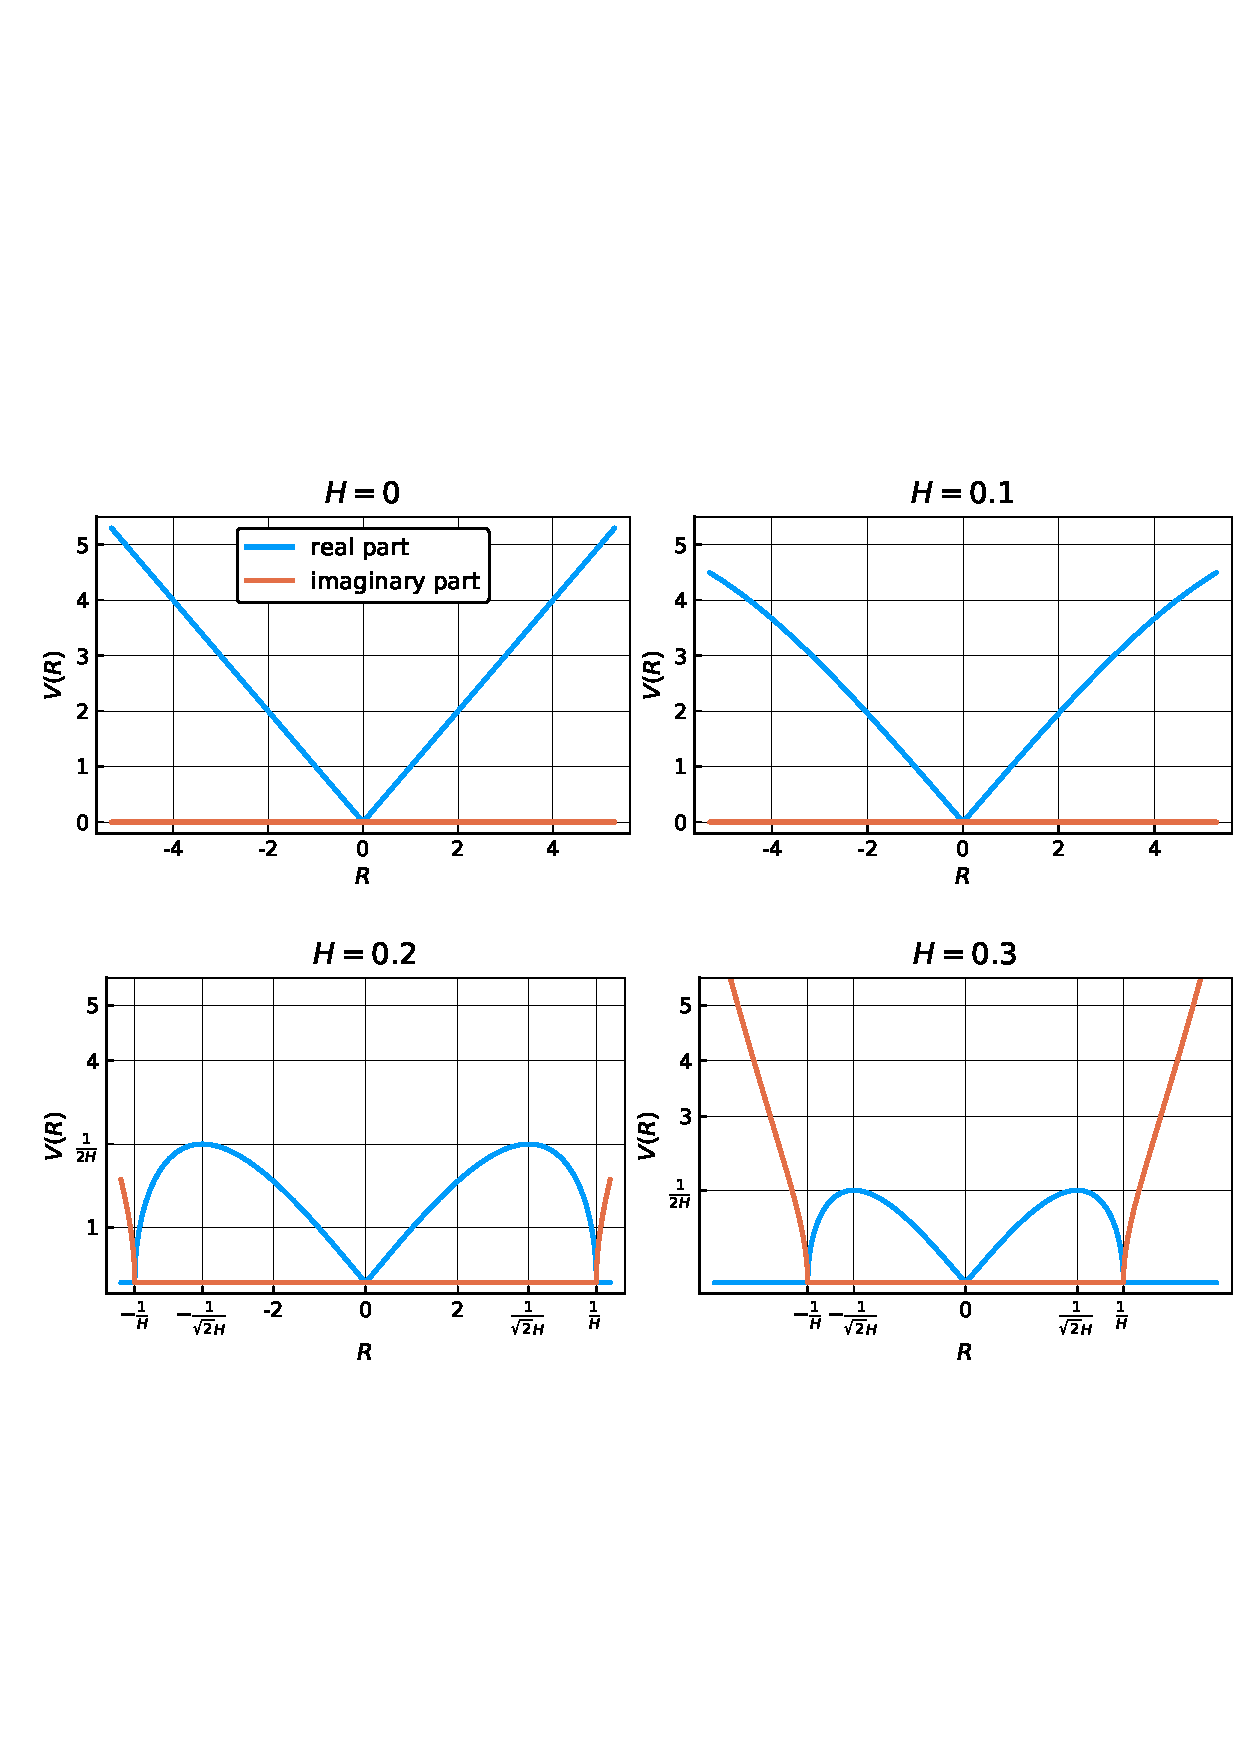
\includegraphics[width=12.5cm]{potential.pdf}}
\end{frame}


\begin{frame}
\frametitle{Flat spacetime}
\vspace*{0.05cm}\hspace*{-0.2cm}\raisebox{0cm}{
	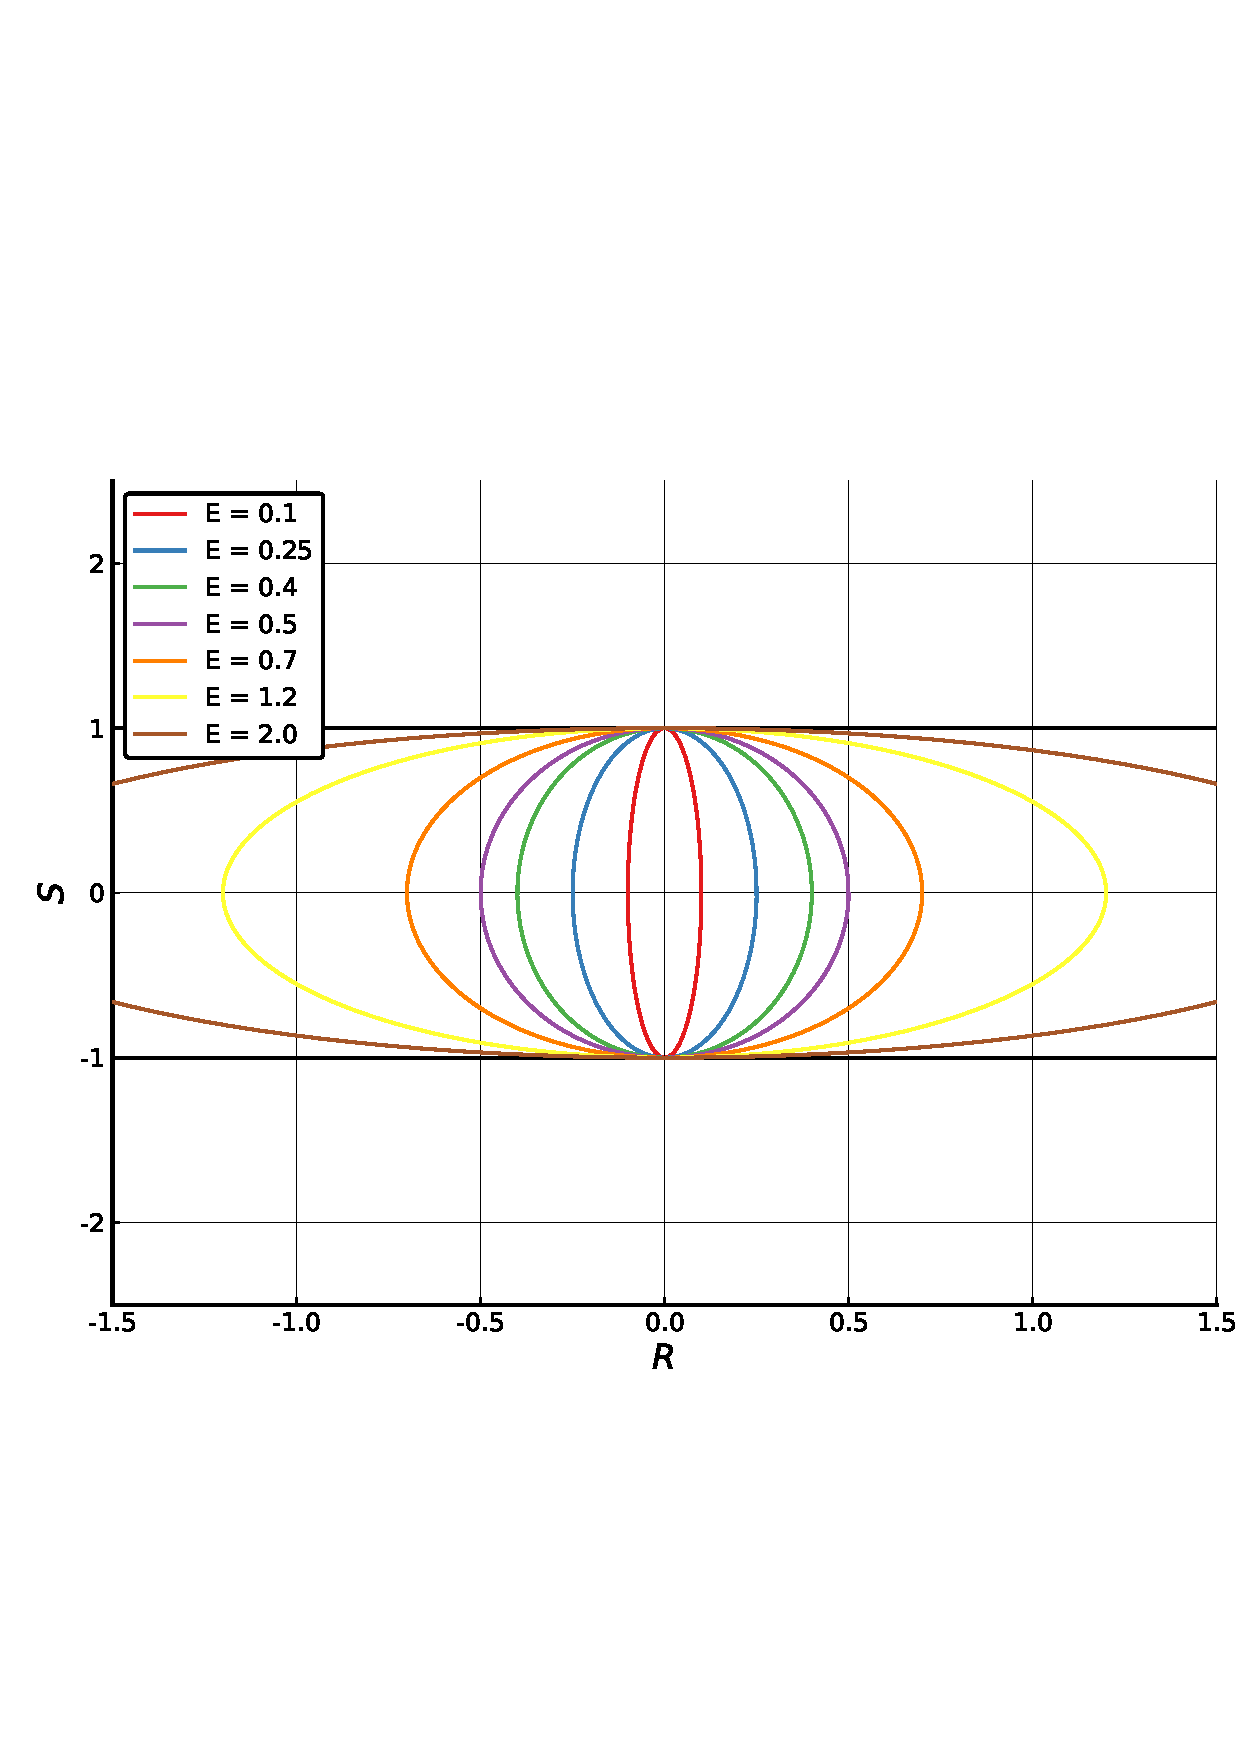
\includegraphics[width=1\textwidth]{Flat_closed.pdf}
}
\end{frame}

\begin{frame}
	\frametitle{Constantly expanding universe -- de~Sitter spacetime}
	\vspace*{0.05cm}\hspace*{-0.2cm}\raisebox{0cm}{
		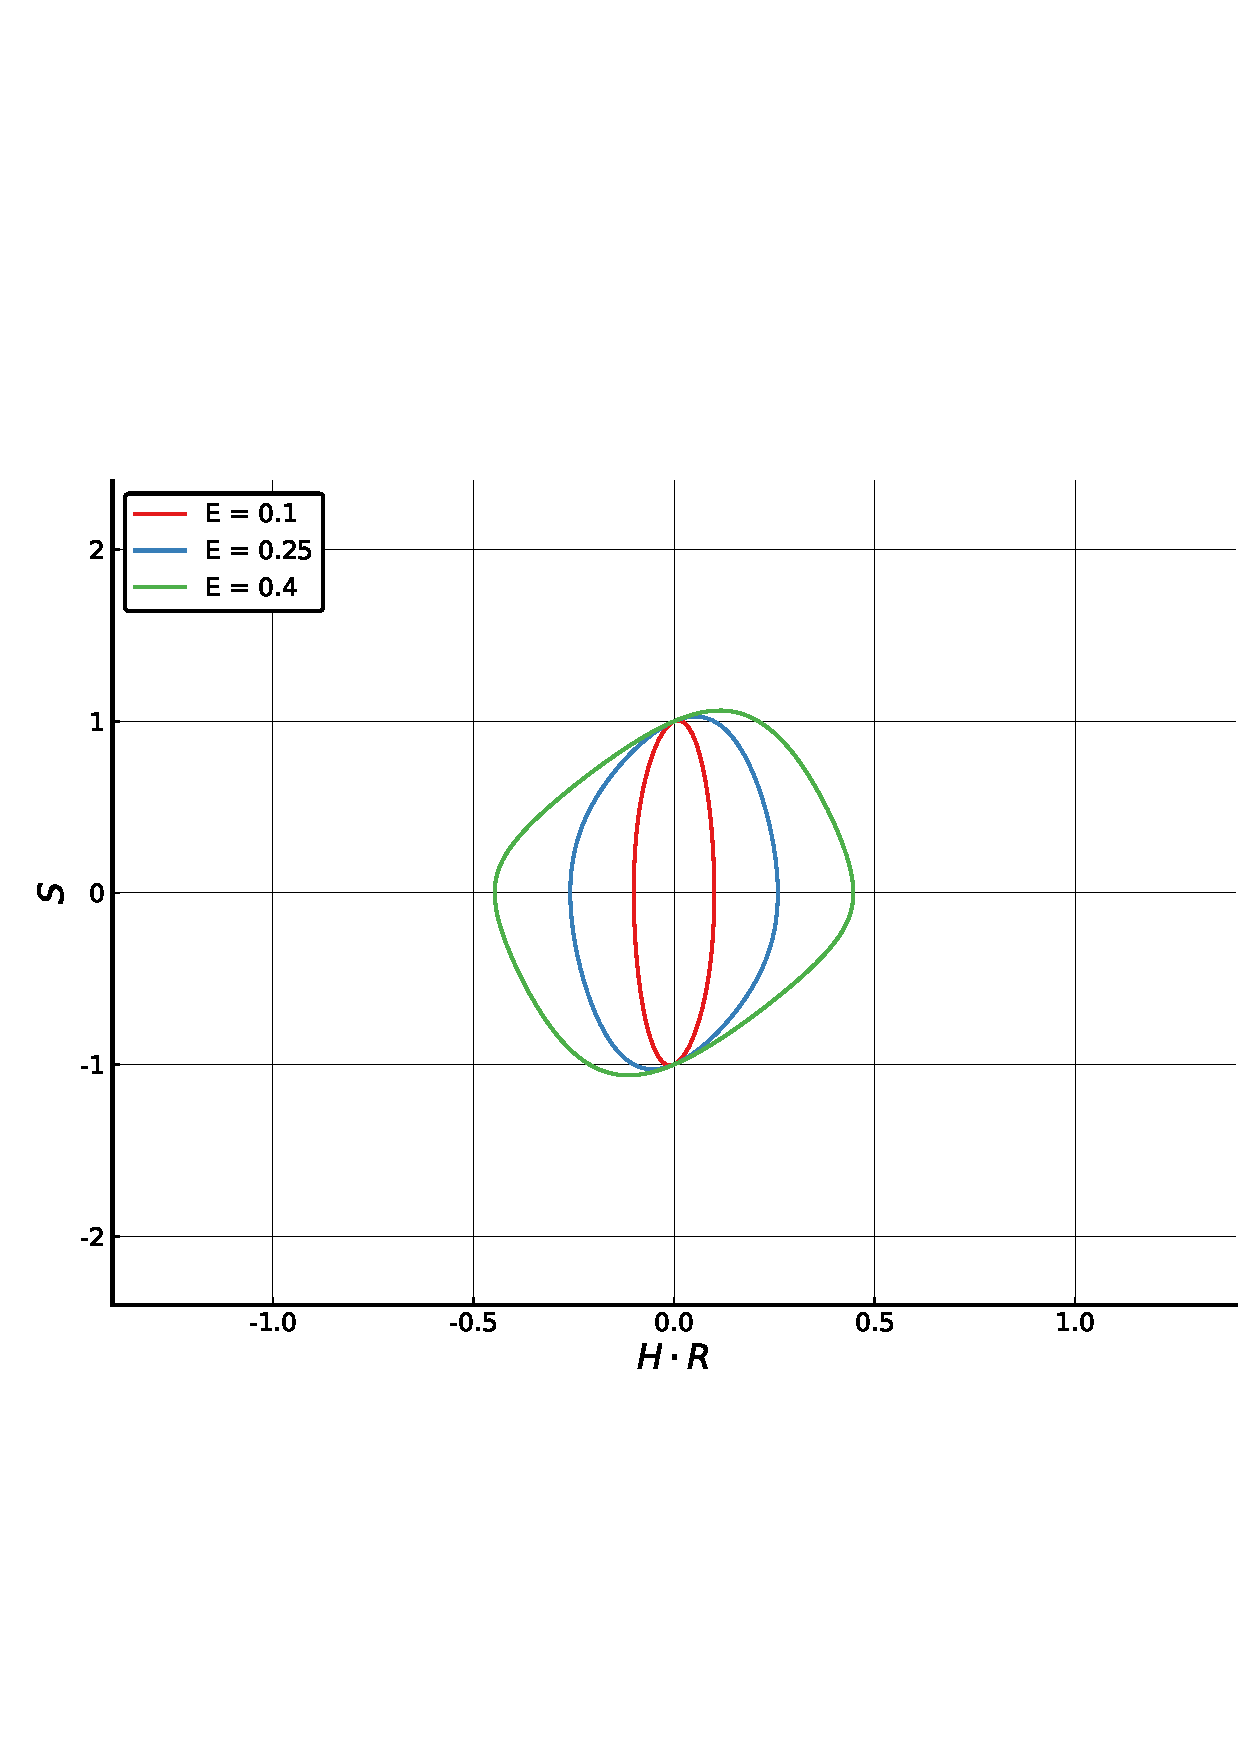
\includegraphics[width=1\textwidth]{DeSitter_closed.pdf}
	}
\end{frame}

\begin{frame}
	\frametitle{Constantly expanding universe -- de~Sitter spacetime}
	\vspace*{0.05cm}\hspace*{-0.2cm}\raisebox{0cm}{
		\includegraphics[width=1\textwidth]{DeSitter_closed_plus_expanding.pdf}
	}
\end{frame}

\begin{frame}
	\frametitle{Constantly expanding universe -- de~Sitter spacetime}
	\vspace*{0.05cm}\hspace*{-0.2cm}\raisebox{0cm}{
		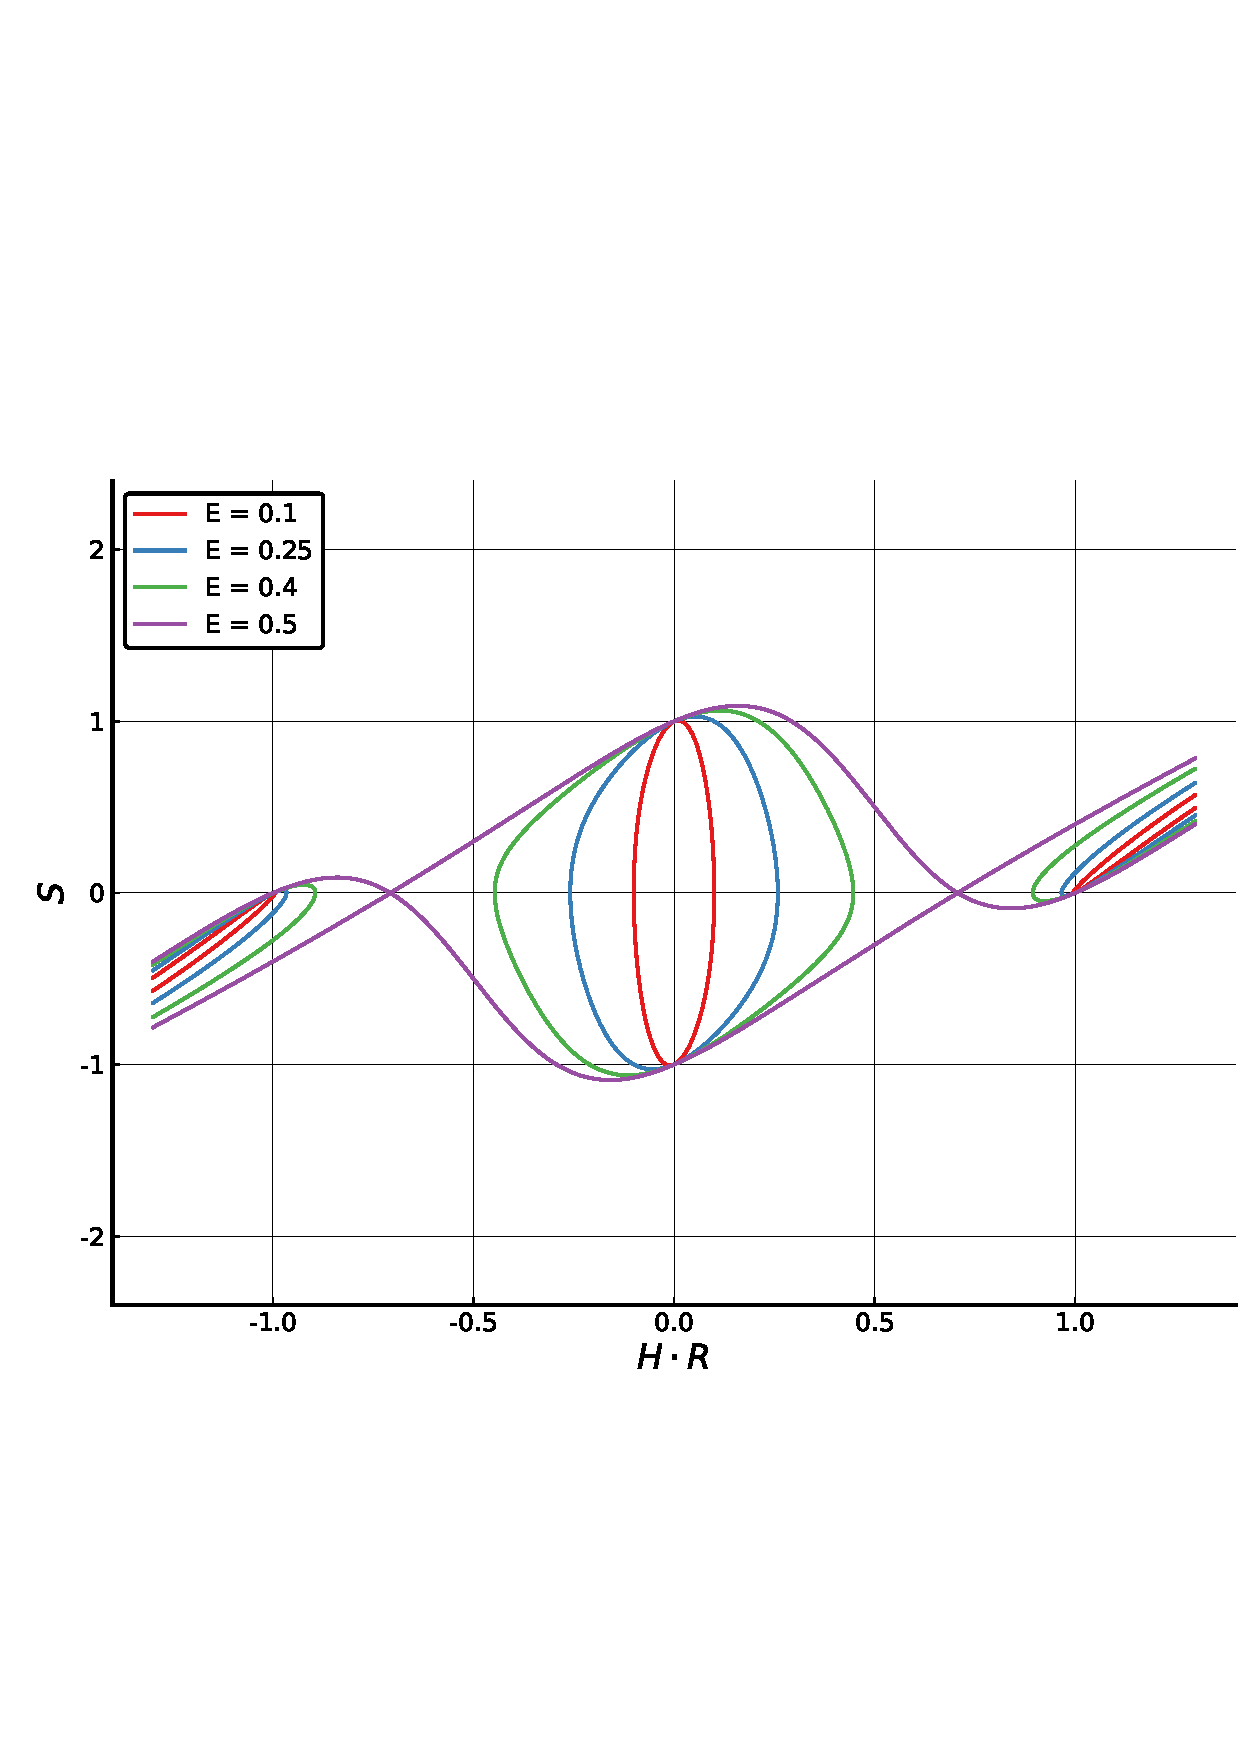
\includegraphics[width=1\textwidth]{DeSitter_labile.pdf}
	}
\end{frame}

\begin{frame}
	\frametitle{Constantly expanding universe -- de~Sitter spacetime}
	\vspace*{0.05cm}\hspace*{-0.2cm}\raisebox{0cm}{
		\includegraphics[width=1\textwidth]{DeSitter_unstable.pdf}
	}
\end{frame}



\begin{frame}[plain]
	%\frametitle{Constantly expanding universe -- de~Sitter spacetime}
	\vspace*{0.0cm}\hspace*{-0.85cm}\raisebox{0cm}{
		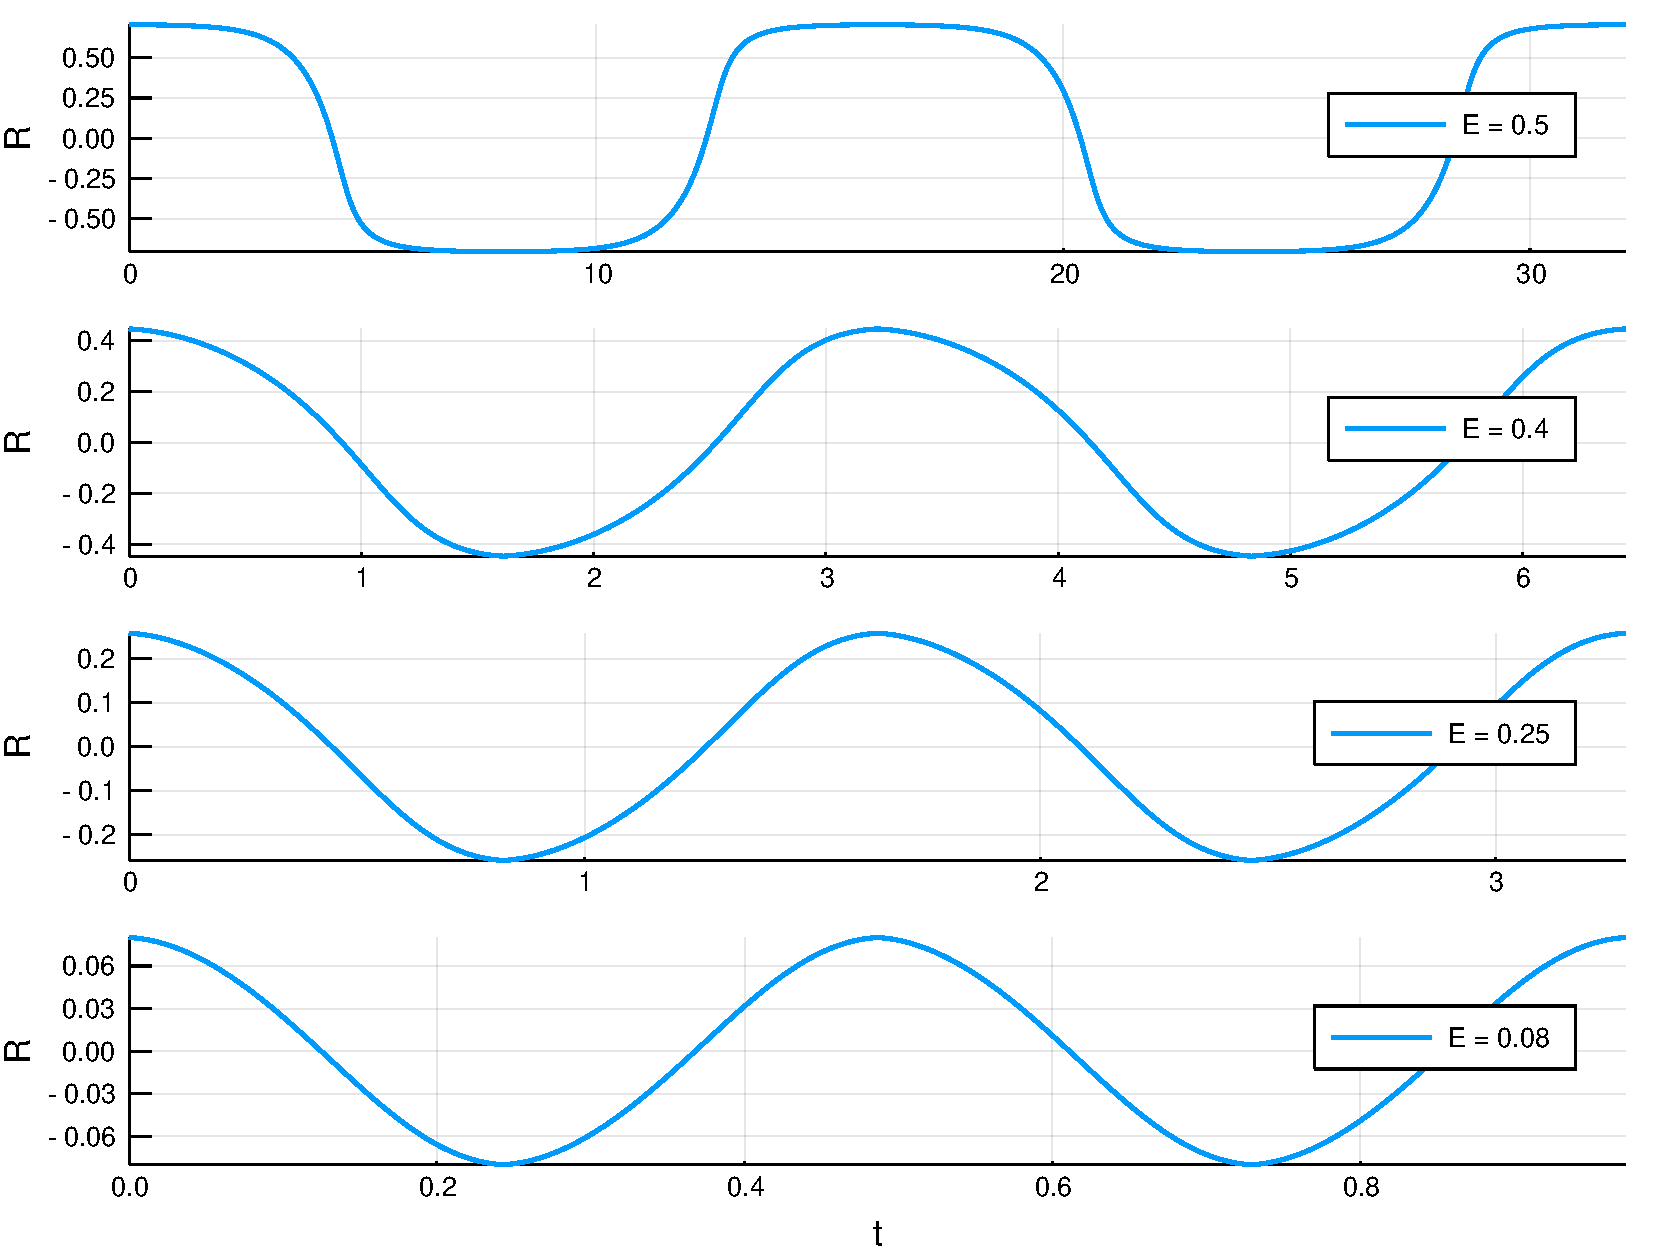
\includegraphics[width=12.3cm]{Time_dep.pdf}
	}
\end{frame}


\section{Gravitational wave background}



\begin{frame}
\frametitle{Gravitational wave background}
\begin{itemize}
	\item Metric takes the form:
	$$
	\D s^2 = H \D u^2 + 2 \D u \D v + \D x^2 + \D y^2
	$$
	where $u = (z+t)/\sqrt{2}$ and $v = (z-t)/\sqrt{2}$
	\item $H = H(u, x, y)$ satisfies
	$$
	\difs[2] H x + \difs[2] H y = 0
	$$
	\pause
	\item Same parameterization conditions as in flat spacetime
	$$
	\gamma_{\tau \tau} + \gamma_{\sigma \sigma} = 0, \qquad \gamma_{\tau \sigma} = \gamma_{\sigma \tau} = 0
	$$
\end{itemize}
\end{frame}



\begin{frame}
	\frametitle{Interaction with gravitational wave burst}
	\begin{itemize}
	\item We choose the gravitational wave function $H$ to be a~gaussian burst with $+$ polarization, frequency $\omega$ and amplitude $A$:
	$$
	H = (x^2 - y^2) h(\tau)
	$$
	\begin{center}
	\includegraphics[width=8cm]{grav_wave_profile.pdf}
	\end{center}
	\item Space is flat in regions long before and long after the gravitational wave burst
	\pause
	\item Similarly to flat spacetime, we can expand the $\sigma$ dependance into modes:
	$$
	X^i(\sigma, \tau) = \sum\limits_{k_i \in \Zbb} X^i_{k_i}(\tau) \me^{2 \pi \mi k_i \sigma/\sigma_1} \qquad i \in \{v, x, y\}
	$$
	\end{itemize}	
\end{frame}

\begin{frame}
	\frametitle{Interaction with gravitational wave burst}
	\begin{itemize}
		\item The $\tau$ evolution of each mode is given by its equation of motion
		$$
		\begin{aligned}
		\lp \difs[2]{}{\tau} + k_x^2 - h(\tau) \rp x_{k_x} = 0 & \\
		\lp \difs[2]{}{\tau} + k_y^2 + h(\tau) \rp y_{k_y} = 0 & \\
		\begin{aligned}
		\lp \difs[2]{}{\tau} + k_v^2 \rp v_{k_v} = \sum\limits_{k_x}  x_{k_x} x_{k_v-k_x} \difs {h(\tau)} {\tau}/2 - 2 x_{k_x} \difs {x_{k_v-k_x}} {\tau} h(\tau) \\
		+ \sum\limits_{k_y}  y_{k_y} y_{k_v-k_y} \difs {h(\tau)} {\tau}/2 - 2 y_{k_y} \difs {y_{k_v-k_y}} {\tau} h(\tau)
		\end{aligned} &
		\end{aligned}
		$$
		\pause
		\item Strong interaction between string and gravitational wave for resonant frequencies
		$$
		\omega \approx \frac{2 \sqrt{2}}{n}, \qquad n \in \Zbb
		$$
	\end{itemize}
\end{frame}



\begin{frame}
\frametitle{Interaction with gravitational wave burst}
	\vspace*{-0.1cm}\hspace*{-1.1cm}\raisebox{-1cm}{
	\begin{tabular}{cc}
		Energy & Velocity $v_z$ \\
		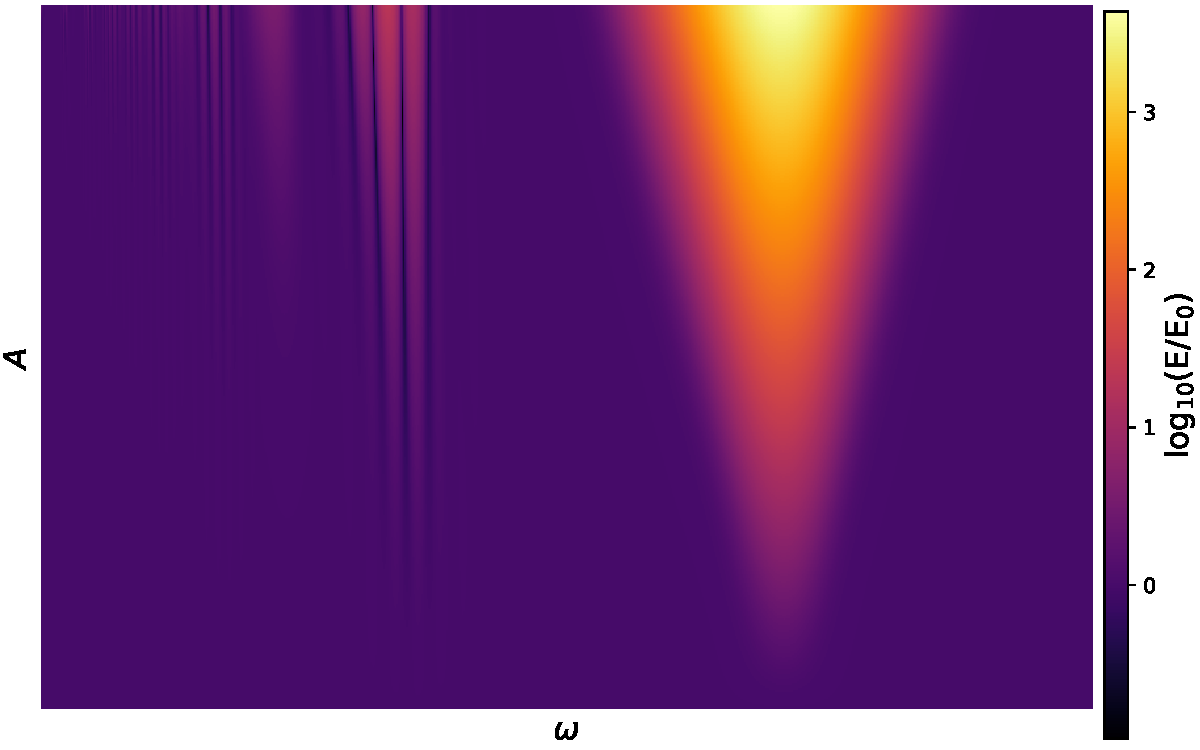
\includegraphics[width=6cm]{grav_energy.png} & \hspace{-0.2cm}
		\includegraphics[width=6cm]{grav_velocity.png} \\ 
		\includegraphics[width=6cm]{grav_energy_small.png} & \hspace{-0.2cm}
		\includegraphics[width=6cm]{grav_velocity_small.png}
	\end{tabular}}\hspace*{12cm}
\end{frame}


\begin{frame}[plain]
	\vspace*{-0.5cm}\hspace*{-1.1cm}\raisebox{-1cm}{
		\animategraphics[autoplay,loop,width = 12.7cm]{25}{string_grav_combined/string_grav_}{1}{1001}}
\end{frame}


\begin{frame}
	\frametitle{Summary}
	\begin{itemize}
		\item Understanding of the gauge choices and some tricks to simplify equations.
		\item Small circular strings in an expanding universe feel little difference from flat spacetime.
		\item Circular strings of cosmological scale in an expanding universe expand to infinity or until they break.
		\item General solution for gravitational wave background.
		\item Interaction of circular string with gravitational wave pulse.
		\item Resonant frequencies between strings and gravitational waves.
	\end{itemize}
\end{frame}

\appendix

\section{Questions}

\begin{frame}
	\frametitle{Oponent's question no. 1}
	\begin{itemize}
		\item 
		Q: In chapter one it is said that to find the equations of motion one has to minimize
		the action. In general one only looks for extrema of the action, which could be a
		minimum, a maximum or a saddle point. Is it clear that in the present context only
		minima arise?
		
		\item A: All types of extrema are possible and physically correct.
	\end{itemize}			
\end{frame}


\begin{frame}
	\frametitle{Oponent's question no. 2}
	\begin{itemize}
		\item Q: In eq. (1.10) the last step is not very obvious to me.
		$$
		\delta (\det \gamma) = \det \gamma \gamma^{\alpha \beta} \delta \gamma_{\alpha \beta} 
		$$
		\item A: Maybe it is better to use the identity
		$$
		\det \lp \me^{A} \rp = \me^{\tr (A)}
		$$
		then we can write
		$$
		\begin{aligned}
		\delta \det \gamma = \delta \det \lp \me^{\ln \gamma} \rp = \delta \me^{\tr \ln \gamma} = \det \gamma \tr \lp \gamma^{-1} \delta \gamma \rp \\
		 = \det \gamma \gamma^{\alpha \beta} \delta \gamma_{\alpha \beta}
		\end{aligned}
		$$
	\end{itemize}
\end{frame}


\begin{frame}
\frametitle{Oponent's question no. 3}
\begin{itemize}
	\item Q: Eqs. \eqref{eq:omega} and \eqref{eq:domega} are incorrect
	\begin{equation}
	\tag{1.19} \label{eq:omega}
	\omega = \sqrt{- \gamma} \gamma^{\alpha \beta} g_{MN} \difs[]{X^M}{\alpha} \delta X^N
	\end{equation}
	\begin{equation}
	\tag{1.20} \label{eq:domega}
	\D \omega = \difs{\lp \sqrt{- \gamma} \gamma^{\alpha \beta} g_{MN} \difs[]{X^M}{\alpha} \delta X^N \rp} {\beta} \D y^{\beta}
	\end{equation}
	\item A: The integral for which we use the Stoke's theorem is
	$$
	\int\limits_{\tau_i}^{\tau_f} \int\limits_{0}^{\sigma_1} \D \tau \D \sigma ~ \difs{\lp \mathcal{P}_N^{\beta} \delta X^N \rp } {\beta} \qquad \mathcal{P}_N^{\beta} = \sqrt{- \gamma} \gamma^{\alpha \beta} g_{MN} \difs[]{X^M}{\alpha}
	$$
	the corresponding 2-form is
	$$
	\D \omega = \left[ \difs{\lp \mathcal{P}_N^{\tau} \delta X^N \rp } {\tau} + \difs{\lp \mathcal{P}_N^{\sigma} \delta X^N \rp } {\sigma} \right] \D \tau \wedge \D \sigma
	$$
	we can see, that this is an exterior derivative of
	$$
	\D \omega = \D {\left[ \mathcal{P}_N^{\tau} \delta X^N \D \sigma - \mathcal{P}_N^{\sigma} \delta X^N \D \tau \right]}
	$$
\end{itemize}
\end{frame}


\begin{frame}
\frametitle{Oponent's question no. 4}
\begin{itemize}
	\item Q: In sec. 2.1 the freedom of reparameterizing the string worldsheet is used to take $t = \tau$
	and impose eq. (2.3) and also $C(\sigma) = 1$. This is three conditions while the freedom
	to make reparameterizations involves two free functions. A comment about why this
	is okay would be useful.
	\item A: Imposing eq. (2.3)
	\begin{equation}\tag{2.3}
		g_{MN} \difs {X^M}{\tau} \difs {X^N}{\sigma} = \gamma_{\tau \sigma} = 0
	\end{equation}
	does not fully specify the parameterization (only that it is perpendicular to the direction of constant lines of $\tau$). And because the quantity
	$$
	C(\sigma) = \sqrt{\frac{\gamma_{\sigma \sigma}}{\gamma_{\tau \tau}}} = \text{const.}
	$$
	we can choose the "length" of $\difs {X^M} {\sigma}$, which corresponds to choosing a specific value for the const.
\end{itemize}
\end{frame}


\begin{frame}
\frametitle{Oponent's question no. 5}
\begin{itemize}
	\item Q: In eq. (2.20) the boundary conditions given are for an open string, without comment.
	While the rest of the thesis seems to be about closed strings, or were open strings
	also considered?
	\item A: The conditions for open strings were for a complete picture. We only studied closed strings, that automatically satisfy these conditions.
\end{itemize}
\end{frame}


\begin{frame}
\frametitle{Oponent's question no. 6}
\begin{itemize}
	\item Q: In sec. 3.1 a coordinate $R = r \me^{Ht}$ is introduced which is positive by definition, but
	then negative values of $R$ are allowed, e.g. Fig. 3.1. What is the reason for this?
	\item A: It is similar to harmonic oscilator -- when the string goes to the point $r = 0$ it reaches maximum velocity $\difs {r} {t}$. The passage through this point would mean either that $r \rightarrow -r$ or $\theta \rightarrow \theta + \pi$
\end{itemize}
\end{frame}


\begin{frame}
\frametitle{Oponent's question no. 7}
\begin{itemize}
	\item Q:  Figures 3.5-10 mention de Sitter space but it is not explained anywhere what this
	space is and how it’s related to the expanding FLRW universe considered.
	\item A: De Sitter space (in 4D) is defined as a submanifold in Minkowski spacetime
	$$
	\D s^2 = -\D t^2 + \D x^2 + \D y^2 + \D z^2
	$$
	that satisfies
	$$
	-t^2 + x^2 + y^2 + z^2 = \alpha^2
	$$
\end{itemize}
\end{frame}


\begin{frame}
\frametitle{Oponent's question no. 7}
	It can be shown, that with the coordinate change 
	$$
	\begin{gathered}
	t = \alpha \sinh \lp \frac{t'}{\alpha} \rp + (y'^2 + z'^2) \frac{\me^{t'/\alpha}}{2 \alpha} \\
	x = \alpha \cosh \lp \frac{t'}{\alpha} \rp - (y'^2 + z'^2) \frac{\me^{t'/\alpha}}{2 \alpha} \\
	y = \me^{t'/\alpha} y' \qquad z = \me^{t'/\alpha} z'
	\end{gathered}
	$$
	the metric becomes
	$$
	\D s^2 = -\D t'^2 + \me^{2t'/\alpha} \lp \D x'^2 + \D y'^2 + \D z'^2 \rp
	$$
	This is the same form as the FLWR metric with only the cosmological constant
\end{frame}


\begin{frame}
\frametitle{Oponent's question no. 8}
\begin{itemize}
	\item Q: Related to point 4. Why are you allowed to impose the condition $u = \lambda \tau$ in (4.15) when you have already imposed two conditions on $\gamma$ in (4.9)?
	\begin{equation} \tag{4.15}
	\begin{aligned}
	\gamma_{\tau \tau} + \gamma_{\sigma \sigma} = 0 \qquad 
	\gamma_{\tau \sigma} = \gamma_{\sigma \tau} = 0 
	\end{aligned}
	\end{equation}
	\item A: In order for the transformations
	$$
	\tau' = \varphi_1(\tau, \sigma), \qquad \sigma' = \varphi_2(\tau, \sigma)
	$$
	to preserve the conditions (4.15), they must satisfy
	$$
	(\difs[2]{}{\tau} - \difs[2]{}{\sigma}) \tau' = 0, \qquad (\difs[2]{}{\tau} - \difs[2]{}{\sigma}) \sigma' = 0
	$$
	Moreover, the second equation of motion reads
	$$
	(\difs[2]{}{\tau} - \difs[2]{}{\sigma}) u = 0,
	$$
	so we can choose $\tau' = u/\lambda$.
\end{itemize}
\end{frame}



\begin{frame}
\frametitle{Oponent's question no. 9}
\begin{itemize}
	\item Q: In chapter 4 it would be nice to indicate the duration of the gravitational wave in
	fig 4.6-7 and to have an explanation in words of what happens to the string when
	the gravitational wave hits and contrasting this with what happens to a point-like
	particle.
	\item A: The $\rho$ parameter that specifies the duration of the pulse had the value $\rho = 10$ in the units of time. The position of the strong interactions for resonant frequencies does not change while varying the length of interaction.
	The animations shown in this presentation should answer the second part of this question. 
\end{itemize}
\end{frame}


\section{Bonus slides}

\begin{frame}[plain]
\hspace*{-1.5cm}\begin{minipage}{0.55\textwidth}
	\includegraphics[width=7.5cm]{Mathieu_stability.PNG} 
\end{minipage} \hfill
\begin{minipage}{0.43\textwidth}
	Taken from \bibentry{lachlan}
\end{minipage}
\end{frame}


\bibliographystyle{unsrt}
\nobibliography{citations}

\end{document} 
